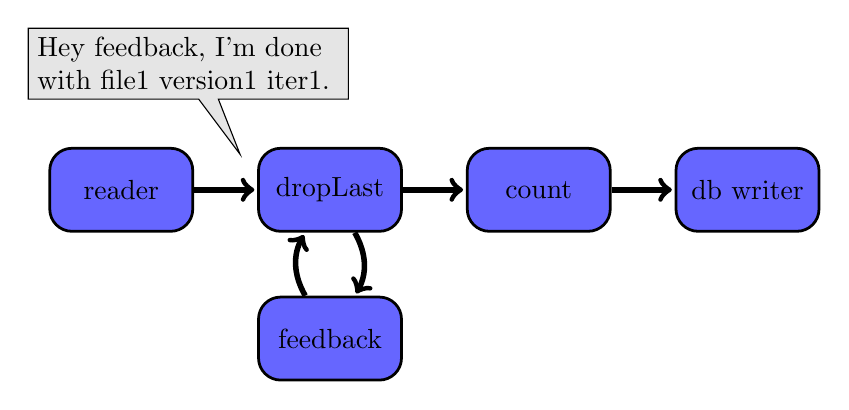
\begin{tikzpicture}[node distance = 0.8cm, auto]
\usetikzlibrary{shapes,arrows}
\usetikzlibrary{positioning}

\tikzstyle{operator} = [rectangle, draw, fill=blue!60, text width=4.5em, text centered, rounded corners = 8pt, minimum height=30pt, line width=1pt]
\tikzstyle{callout} = [draw, rectangle callout, callout relative pointer={#1}, line width=1pt]

    \node [operator] at (0, 0) (reader) {reader};
    \node [operator, right = of reader] (filter) {dropLast};
    \node [operator, right = of filter] (count) {count};
    \node [operator, below = of filter] (feedback) {feedback};
   \node[draw, rectangle callout,callout relative pointer={(0.4cm,-0.7cm)}, shift={(-1.8,-0.2)},  text width=10.9em, aspect=2.5,fill=black!10, above = of filter] (hello) {Hey feedback, I'm done with file1 version1 iter1.};
    \node [operator, right = of count] (writer) {db writer};


    \draw [thick,->,shorten >=1pt, line width=2pt] (reader) -- (filter) ;
    \draw [thick,->,shorten >=1pt, line width=2pt] (filter) -- (count); 
     \draw [thick,->,shorten >=1pt, line width=2pt] (count) -- (writer); 
    \draw [thick,->,shorten >=1pt, line width=2pt] (filter) to  [bend left]  (feedback); 
     \draw [thick,->,shorten >=1pt, line width=2pt] (feedback) edge  [bend left]  (filter); 
\end{tikzpicture}
